\newpage
\section {Билет 4. Индексы (дерево, карты, хэш).}

Индекс применяется для ускорения поиска нужных строк (в операциях
выборки/обновления/удаления). Индекс является упорядоченной структурой (записи в индексе хранятся в отсортированном виде). После создания индекса в актуальном состояние его поддерживает СУБД.

По умолчанию команда CREATE INDEX создаёт индексы-B-деревья, эффективные в большинстве случаев. Выбрать другой тип можно, написав название типа индекса после ключевого слова USING. 

\textbf{B-дерева:} 

Свойства B-дерева: 
\begin{itemize}
	\item В каждом узле заполнено от k/2 до k значения. Корень содержит 1 до k ключей.
	\item Все листья B-дерева должны быть расположены на одной высоте, которая и является высотой дерева.
	\item У листьев потомков нет. Любой другой узел, содержащий ключи $K_{1}, …,  K_{n}$ содержит $n+1$ потомков. При этом:
	
	1. Первый потомок и все его потомки содержат ключи из интервала  $(-\infty ,K_{1})$
	
	2. Для $ 2\leq i\leq n$ n, i-й потомок и все его потомки содержат ключи из интервала $ (K_{i-1},K_{i})$ 
	
	3. $(n+1)-$й потомок и все его потомки содержат ключи из интервала $(K_{n},\infty )$
\end{itemize}


B-деревья могут работать в условиях на равенство и в проверках диапазонов с данными, которые можно отсортировать в некотором порядке. Точнее, планировщик запросов PostgreSQL может задействовать индекс-B-дерево, когда индексируемый столбец участвует в сравнении 

\textit{Недостатки}: поиск только по одному столбцу. (Если нам нужно найти брюнетов с зелеными глазами, то по дереву мы найдем брюнетов, а дальше уже придется проверять их всех, то есть не использовать индексы)

\textbf{Bitmap(карты)} 

В bitmap-структурах создается двухмерный массив со столбцом для каждой строки в индексируемой таблице. Каждый столбец представляет отдельное значение в bitmap-индексе. Этот двухмерный массив показывает каждое значение индекса, умноженное на количество строк в этой таблице.

Пример поиска по индексу на рисунке (он приводил похожий, но на конкретном примере): 
\begin{figure}[H]
	\centering
	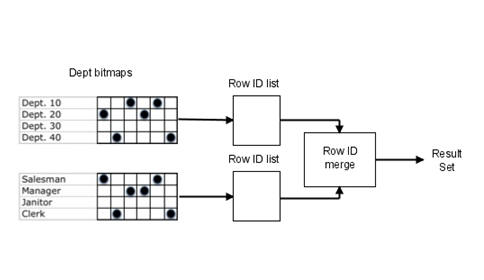
\includegraphics[scale = 0.3]{4/Map.jpeg}
\end{figure}

Берем строчку из первого индекса (по условиям нашим), и строчку из второго индекса. Дальше логические операции заменяем на побитовые и проводим их на наших выбранных строчках. 

\textit{Недостатки:} Предположим, мы заблокировали запись -> нужно заблокировать часть индекса, где она участвует (в дереве - только лист, там мало значений: k), а вот у карты нужно блокировать всю строку индекса - это много.

\textbf{Хеш - индексы} 

Просто по значениям в таблице вычисляем некоторую хеш функцию и значения таблицы помещаем в ячейку с номером хеша. 

Хеш - индекс детально не рассматривали. 